\chapter{SETTING COORDINATE FRAMES}
    \section{Topic}
        \hspace*{0.6cm}Set coordinate frames for the first four links (link 1, link 2, link 3).
    \section{Theory}
    \hspace*{0.6cm}Based on “DENAVIT-HARTENBERG NOTATION” (Lecture 4: Forward Kinematics [1]): Local frame \textbf{$B_i$} to each link (i) at joint $i+1$ is defined as:
    \begin{itemize}
        \item The $z_i$ axis is aligned with the $i + 1$ joint axis.
        \item The $x_i$ axis is defined along the common normal between the $z_i - 1$ and $z_i$
        axes, pointing from the $z_i - 1$ to the $z_i$ axis.
        \item The $y_i$ axis is defined by the right-hand rule.
        \item The origin $o_i$ of the $i$ frame is located at the intersection of the joint axis $i+1$ with the common normal between the $z_i - 1$ and $z_i$ axes.
    \end{itemize}

    \section{Application}
    \begin{figure}[H]
        \centering
        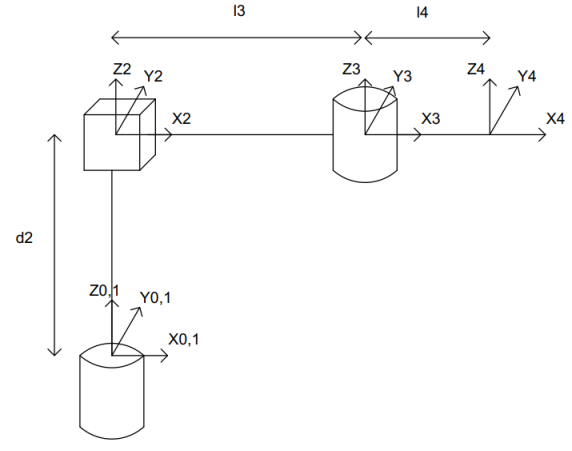
\includegraphics[width=0.7\textwidth]{pictures/set_frame.png} 
        \caption{Setting coordinate frames for robot}
    \end{figure}

            Phương trình Lagrange tổng quát cho cơ hệ
            \begin{align}
                \frac{d}{dt} \left( \frac{\partial L}{\partial \dot{q_i}} \right) - \frac{\partial L}{\partial q_i} = Q_i
            \end{align}

            Trong đó
            \begin{itemize}
                \item $L = K - V$: hàm Lagrange
                \item $q_i$: tọa độ suy rộng, trong phạm vi bài báo cáo ta có $q = [x \,\, \theta]^T$
                \item $\dot{q_i}$: đạo hàm theo thời gian của $q_i$
                \item $Q_i$: moment hoặc lực tổng quát (nếu có). Trong phạm vi bài báo cáo ta có $Q_i = [F_x \,\, \tau_\theta]$.
            \end{itemize}

            Hàm Lagrange
            \begin{align}
                L = K - V = \dfrac{1}{2} M_{\Sigma} \dot{x}^2 + \dfrac{1}{2} J \dot{\theta}^2 + M_p \ell \dot{x} \dot{\theta} \cos \theta - M_p g \ell \cos \theta 
            \end{align}    

            Đối với tọa độ suy rộng $x$:
            \begin{align*}
                &\frac{\partial L}{\partial \dot{x}} = M_{\Sigma} \dot{x} + M_p \ell \dot{\theta} \cos \theta\\
                &\frac{d}{dt} \left( \frac{\partial L}{\partial \dot{x}} \right) = M_{\Sigma} \ddot{x} + M_p \ell \ddot{\theta} \cos \theta - M_p \ell \dot{\theta}^2 \sin \theta\\
                &\frac{\partial L}{\partial x} = 0
            \end{align*}

            Do đó
            \begin{align}
                M_{\Sigma} \ddot{x} + M_p \ell \ddot{\theta} \cos \theta - M_p \ell \dot{\theta}^2 \sin \theta = F_x
            \end{align}


            Đối với tọa độ suy rộng $\theta$:
            \begin{align*}
                &\frac{\partial L}{\partial \dot{\theta}} = J \dot{\theta} + M_p \ell \dot{x} \cos \theta\\
                &\frac{d}{dt} \left( \frac{\partial L}{\partial \dot{\theta}} \right) = J \ddot{\theta} + M_p \ell \ddot{x} \cos \theta - M_p \ell \dot{x} \dot{\theta} \sin \theta\\
                &\frac{\partial L}{\partial \theta} = -M_p \ell \dot{x} \dot{\theta} \sin \theta - M_p g \ell (-\sin \theta) = -M_p \ell \dot{x} \dot{\theta} \sin \theta + M_p g \ell \sin \theta
            \end{align*}

            Do đó
            \begin{align}
                J \ddot{\theta} + M_p \ell \ddot{x} \cos \theta - M_p \ell \dot{x} \dot{\theta} \sin \theta + M_p \ell \dot{x} \dot{\theta} \sin \theta - M_p g \ell \sin \theta = \tau_\theta \nonumber\\
                \Leftrightarrow J \ddot{\theta} + M_p \ell \ddot{x} \cos \theta - M_p g \ell \sin \theta = \tau_\theta
            \end{align}

            Từ phương trình (1.13) và (1.15) ta có hệ 

            \begin{equation}
                \begin{cases}
                    M_{\Sigma} \ddot{x} + M_p \ell \ddot{\theta} \cos \theta - M_p \ell \dot{\theta}^2 \sin \theta = F_x \\
                    J \ddot{\theta} + M_p \ell \ddot{x} \cos \theta - M_p g \ell \sin \theta = \tau_\theta
                \end{cases}
            \end{equation}

            Ta đưa về dạng tổng quát
            \begin{equation}
                M(q) \ddot{q} + C (q, \dot{q}) \dot{q} + G(q) = \tau
            \end{equation}
            Trong đó
            \begin{itemize}
                \item $q = [x \,\, \theta]^T$: vector trạng thái
                \item $M(q)$: ma trận quán tính
                \item $C(q, \dot{q})$: ma trận Coriolis và ly tâm
                \item $G(q)$: vector trọng lực
                \item $\tau$: moment xoắn điều khiển từ động cơ
            \end{itemize} 
            Ta được
            \begin{align*}
                &\underbrace{
                \begin{bmatrix}
                M_\Sigma & M_p \ell \cos \theta\\
                M_p \ell  \cos \theta & J
                \end{bmatrix}
                }_{M(q)}
                \begin{bmatrix}
                \ddot{x} \\ \ddot{\theta}
                \end{bmatrix}
                +
                \underbrace{
                \begin{bmatrix}
                0 & -M_p \ell \dot{\theta} \sin \theta \\
                0 & 0
                \end{bmatrix}
                }_{C(q, \dot{q})}
                \begin{bmatrix}
                \dot{x} \\ \dot{\theta}
                \end{bmatrix} 
                +
                \underbrace{
                \begin{bmatrix}
                0 \\
                -M_p g \ell \sin \theta
                \end{bmatrix}
                }_{G(q)}
                =
                \underbrace{
                \begin{bmatrix}
                F_x \\
                \tau
                \end{bmatrix}
                }
            \end{align*}
        
        Trong chương tiếp theo, ta sẽ tiến hành thiết kế và mô phỏng các bộ điều khiển dựa trên hàm truyền đã thu được.
            
        
       